% vim: set textwidth=120:

% Example CV based on the 1.5-column-cv template. Main features:
% * uses the Roboto font family and IcoMoon icon set;
% * doesn't use colours, different font weights are used instead for styling;
% * because the CV fits on one page, header and footer is empty, since there isn't much useful info to put there;
% * includes a photo.
\documentclass[a4paper,10pt]{article}


% package imports
% ---------------

\usepackage[british]{babel} % for correct language and hyphenation and stuff
\usepackage{calc}           % for easier length calculations (infix notation)
\usepackage{enumitem}       % for configuring list environments
\usepackage{fancyhdr}       % for setting header and footer
\usepackage{fontspec}       % for fonts
\usepackage{geometry}       % for setting margins (\newgeometry)
\usepackage{graphicx}       % for pictures
\usepackage{microtype}      % for microtypography stuff
\usepackage{xcolor}         % for colours
\usepackage{datetime}
\usepackage{hyperref}
\usepackage{shadowtext}



% margin and column widths
% ------------------------

% margins
\newgeometry{left=8mm,right=15mm,top=15mm,bottom=15mm}

% width of the gap between left and right column
\newlength{\cvcolumngapwidth}
\setlength{\cvcolumngapwidth}{3.5mm}

% left column width
\newlength{\cvleftcolumnwidth}
\setlength{\cvleftcolumnwidth}{42.5mm}

% right column width
\newlength{\cvrightcolumnwidth}
\setlength{\cvrightcolumnwidth}{\textwidth-\cvleftcolumnwidth-\cvcolumngapwidth}

% set paragraph indentation to 0, because it screws up the whole layout otherwise
\setlength{\parindent}{0mm}


% style definitions
% -----------------
% style categories explanation:
% * \cvnameXXX is used for the name;
% * \cvsectionXXX is used for section names (left column, accompanied by a horizontal rule);
% * \cvtitleXXX is used for job/education titles (right column);
% * \cvdurationXXX is used for job/education durations (left column);
% * \cvheadingXXX is used for headings (left column);
% * \cvmainXXX (and \setmainfont) is used for main text;
% * \cvruleXXX is used for the horizontal rules denoting sections.

% font families
\defaultfontfeatures{Ligatures=TeX} % reportedly a good idea, see https://tex.stackexchange.com/a/37251

% Configure a directory location for fonts(default: 'fonts/')
\newcommand*{\fontdir}[1][fonts/]{\def\@fontdir{#1}}
\fontdir


\newfontfamily{\cvnamefont}{Roboto Medium}
\newfontfamily{\cvsectionfont}{Roboto Medium}
\newfontfamily{\cvtitlefont}{Roboto Regular}
\newfontfamily{\cvdurationfont}{Roboto Light Italic}
\newfontfamily{\cvheadingfont}{Roboto Regular}
\newfontfamily{\cvhonorfont}{Roboto Medium}
\newfontfamily{\cvboldfont}[Path=\@fontdir,Scale=1]{OpenSans-SemiBold}
\newfontfamily{\cvskillfont}[Path=\@fontdir,Scale=1]{OpenSans-SemiBoldItalic}
\setmainfont{Roboto Light}

% colours
\definecolor{cvnamecolor}{HTML}{000000}
\definecolor{cvsectioncolor}{HTML}{3366ff}
\definecolor{cvtitlecolor}{HTML}{000000}
\definecolor{cvdurationcolor}{HTML}{000000}
\definecolor{cvheadingcolor}{HTML}{000000}
\definecolor{cvmaincolor}{HTML}{000000}
\definecolor{cvrulecolor}{HTML}{000000}
\definecolor{cvwhatcolor}{HTML}{5588ff}
\definecolor{cvwherecolor}{HTML}{656565}
\definecolor{cvnoskillcolor}{HTML}{d9d9d9}
\definecolor{cvboldcolor}{HTML}{808080}
\definecolor{cvskilledcolor}{HTML}{668cff}
\color{cvmaincolor}

% styles
\newcommand{\cvnamestyle}[1]{{\Large\cvnamefont\textcolor{cvnamecolor}{#1}}}
\newcommand{\cvsectionstyle}[1]{{\normalsize\cvsectionfont\textcolor{cvsectioncolor}{#1}}}
\newcommand{\cvtitlestyle}[1]{{\large\cvtitlefont\textcolor{cvtitlecolor}{#1}}}
\newcommand{\cvdurationstyle}[1]{{\small\cvdurationfont\textcolor{cvdurationcolor}{#1}}}
\newcommand{\cvheadingstyle}[1]{{\normalsize\cvheadingfont\textcolor{cvheadingcolor}{#1}}}
\newcommand{\cvboldstlye}[1]{{\normalsize\cvboldfont\textcolor{cvboldcolor}{\scalebox{.93}[1.0]{#1}}}}
\newcommand{\cvskillstlye}[1]{{\normalsize\cvskillfont\textcolor{cvwherecolor}{\scalebox{.95}[1.0]{#1}}}}

% Date time format
\newdateformat{monthyeardate}{%
  \THEDAY \space \monthname[\THEMONTH] \THEYEAR}


% inter-item spacing
% ------------------

% vertical space after personal info and standard CV items
\newlength{\cvafteritemskipamount}
\setlength{\cvafteritemskipamount}{5mm plus 1.25mm minus 1.25mm}

% vertical space after other items
\newlength{\cvafterotheritemskipamount}
\setlength{\cvafterotheritemskipamount}{2mm plus 1mm minus 1mm}


% vertical space after sections
\newlength{\cvaftersectionskipamount}
\setlength{\cvaftersectionskipamount}{1mm plus 0.5mm minus 0.5mm}

% extra vertical space to be used when a section starts with an item with a heading (e.g. in the skills section),
% so that the heading does not follow the section name too closely
\newlength{\cvbetweensectionandheadingextraskipamount}
\setlength{\cvbetweensectionandheadingextraskipamount}{1mm plus 0.25mm minus 0.25mm}


% intra-item spacing
% ------------------

% vertical space after name
\newlength{\cvafternameskipamount}
\setlength{\cvafternameskipamount}{3mm plus 0.75mm minus 0.75mm}

% vertical space after personal info lines
\newlength{\cvafterpersonalinfolineskipamount}
\setlength{\cvafterpersonalinfolineskipamount}{2mm plus 0.5mm minus 0.5mm}

% vertical space after titles
\newlength{\cvaftertitleskipamount}
\setlength{\cvaftertitleskipamount}{1mm plus 0.25mm minus 0.25mm}

% value to be used as parskip in right column of CV items and itemsep in lists (same for both, for consistency)
\newlength{\cvparskip}
\setlength{\cvparskip}{0.5mm plus 0.125mm minus 0.125mm}

% set global list configuration (use parskip as itemsep, and no separation otherwise)
\setlist{parsep=0mm,topsep=0mm,partopsep=0mm,itemsep=\cvparskip}


% CV commands
% -----------

% creates a "personal info" CV item with the given left and right column contents, with appropriate vertical space after
% @param #1 left column content (should be the CV photo)
% @param #2 right column content (should be the name and personal info)
\newcommand{\cvpersonalinfo}[2]{
    % left and right column
    \begin{minipage}[t]{\cvleftcolumnwidth}
        \vspace{0mm} % XXX hack to align to top, see https://tex.stackexchange.com/a/11632
        \raggedleft #1
    \end{minipage}% XXX necessary comment to avoid unwanted space
    \hspace{\cvcolumngapwidth}% XXX necessary comment to avoid unwanted space
    \begin{minipage}[t]{\cvrightcolumnwidth}
        \vspace{0mm} % XXX hack to align to top, see https://tex.stackexchange.com/a/11632
        #2
    \end{minipage}

    % space after
    \vspace{\cvafteritemskipamount}
}

% typesets a name, with appropriate vertical space after
% @param #1 name text
\newcommand{\cvname}[1]{
    % name
    \cvnamestyle{#1}

    % space after
    \vspace{\cvafternameskipamount}
}

% typesets a line of personal info beginning with an icon, with appropriate vertical space after
% @param #1 parameters for the \includegraphics command used to include the icon
% @param #2 icon filename
% @param #3 line text
\newcommand{\cvpersonalinfolinewithicon}[3]{
    % icon, vertically aligned with text (see https://tex.stackexchange.com/a/129463)
    \raisebox{.5\fontcharht\font`E-.5\height}{\includegraphics[#1]{#2}}
    % text
    #3

    % space after
    \vspace{\cvafterpersonalinfolineskipamount}
}

% creates a "section" CV item with the given left column content, a horizontal rule in the right column, and with
% appropriate vertical space after
% @param #1 left column content (should be the section name)
\newcommand{\cvsection}[1]{
    % left and right column
    \begin{minipage}[t]{\cvleftcolumnwidth}
        \raggedleft\cvsectionstyle{#1}
    \end{minipage}% XXX necessary comment to avoid unwanted space
    \hspace{\cvcolumngapwidth}% XXX necessary comment to avoid unwanted space
    \begin{minipage}[t]{\cvrightcolumnwidth}
        \textcolor{cvrulecolor}{\rule{\cvrightcolumnwidth}{0.3mm}}
    \end{minipage}

    % space after
    \vspace{\cvaftersectionskipamount}
}

% creates a standard, multi-purpose CV item with the given left and right column contents, parskip set to cvparskip
% in the right column, and with appropriate vertical space after
% @param #1 left column content
% @param #2 right column content
\newcommand{\cvitem}[2]{
    % left and right column
    \begin{minipage}[t]{\cvleftcolumnwidth}
        \raggedleft #1
    \end{minipage}% XXX necessary comment to avoid unwanted space
    \hspace{\cvcolumngapwidth}% XXX necessary comment to avoid unwanted space
    \begin{minipage}[t]{\cvrightcolumnwidth}
        \setlength{\parskip}{\cvparskip} #2
    \end{minipage}

    % space after
    \vspace{\cvafteritemskipamount}
}

\newcommand{\cvhonoritem}[2]{
    % left and right column
    \begin{minipage}[t]{\cvleftcolumnwidth}
        \raggedleft #1
    \end{minipage}% XXX necessary comment to avoid unwanted space
    \hspace{\cvcolumngapwidth}% XXX necessary comment to avoid unwanted space
    \begin{minipage}[t]{\cvrightcolumnwidth}
        \setlength{\parskip}{\cvparskip} #2
    \end{minipage}

    % space after
    \vspace{1.7mm}
}


\newcommand{\cvotheritem}[2]{
    % left and right column
    \begin{minipage}[t]{\cvleftcolumnwidth}
        \raggedleft #1
    \end{minipage}% XXX necessary comment to avoid unwanted space
    \hspace{\cvcolumngapwidth}% XXX necessary comment to avoid unwanted space
    \begin{minipage}[t]{\cvrightcolumnwidth}
        \setlength{\parskip}{\cvparskip} #2
    \end{minipage}

    % space after
    \vspace{\cvafterotheritemskipamount}
}
% typesets a title, with appropriate vertical space after
% @param #1 title text
\newcommand{\cvtitle}[1]{
    % title
    \cvtitlestyle{#1}

    % space after
    \vspace{\cvaftertitleskipamount}
    % XXX need to subtract cvparskip here, because it is automatically inserted after the title "paragraph"
    \vspace{-\cvparskip}
}

% cv Skill Bar
\makeatletter
\newdimen\skillb@level
\newdimen\skillb@length
\newdimen\skillb@height
\skillb@length=89pt%
\skillb@height=8pt%
\newcommand*{\skillbar}[1]{%
    \skillb@level=\dimexpr#1\skillb@length/100\relax%
    {\color{cvskilledcolor}\rule{\skillb@level}{\skillb@height}}%
    {\color{cvnoskillcolor}%
        \rule{\dimexpr\skillb@length-\skillb@level\relax}{\skillb@height}}%

}
\makeatother

% header and footer
% -----------------

% set empty header and footer
\pagestyle{empty}



% preamble end/document start
% ===========================

\begin{document}



% personal info
% -------------

\cvpersonalinfo{
    % photo
    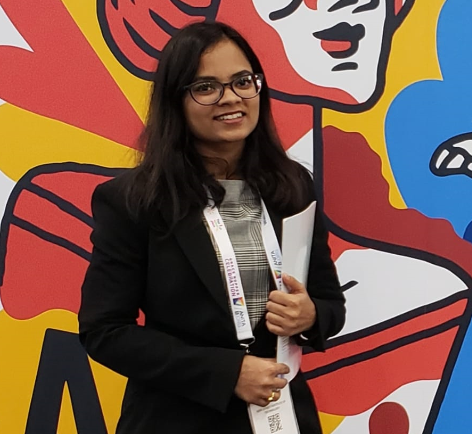
\includegraphics[height=36.5mm]{Profile picture.PNG}
    }{
    % name
    \cvname{Ridhima Shinde}

    % address
    \cvpersonalinfolinewithicon{height=4mm}{072-location.pdf}{
        New Jersey, NJ, 07029 
    }

    % phone number
    \cvpersonalinfolinewithicon{height=4mm}{067-phone.pdf}{
        +1 330-617-2117
    }

    % email address
    \cvpersonalinfolinewithicon{height=4mm}{070-envelop.pdf}{
        \href{mailto:shinderidhima23@gmail.com}{shinderidhima23@gmail.com}
    }

    % LinkedIn account
    \cvpersonalinfolinewithicon{height=4mm}{458-linkedin.pdf}{
        \href{https://www.linkedin.com/in/ridhima-shinde/}{ridhima-shinde}
    }
 
    
   
    
}

% skills
% ------

\cvsection{\textbf{SKILLS}}

\vspace{\cvbetweensectionandheadingextraskipamount}


%  skills
\cvitem{
    \cvheadingstyle{Statistical Programming Languages}
    
}{  
        \setlength\tabcolsep{5pt}
        \begin{tabular}{|l|l|l|l|}

        Python   & R   & SQL    \\
        \footnotesize{\emph{numpy, pandas }} &
        \footnotesize{\emph{RStudio }} &
        \footnotesize{\emph{SSMS, MongoDB}}\\
        
     
         
         
        \end{tabular}
}

% completely vetted skills
\vspace{-2mm}
\cvitem{
    \cvheadingstyle{Other Tools}
    
}{  
        \setlength\tabcolsep{5pt}
        \begin{tabular}{|l|l|l|l|}
        BI Tools  & Cloud Platforms & Reporting+Reporting \\
         \footnotesize{\emph{Tableau, Alteryx}} &
         \footnotesize{\emph{GCP, AWS EC2}} &
         \footnotesize{\emph{Advanced Excel, Salesforce}} 
 %        \footnotesize{\emph{Hadoop, oozie, Scala }}\\
 %        
 %       \footnotesize{\emph{Code Deploy, Code Commit }} &
 %        \footnotesize{\emph{Docker, Amazon EMR }} &
 %        \footnotesize{\emph{Yarn, Postmates}} &
 %        \footnotesize{\emph{RapidMiner}}\\
         
         
         
        \end{tabular}
 }       

 



% work experience
% ---------------

\cvsection{\textbf{WORK EXPERIENCE}}

% Company 1 current
\cvitem{
    \cvdurationstyle{September 2018 -- May 2019}
}{
    \cvtitle{DATA SCIENCE CANDIDATE }

    \textcolor{cvwhatcolor}{\emph{\textbf{OUTREACH ASSISTANT FOR WOMEN IN COMPUTING}}}
    \textcolor{cvwherecolor}{\textbf{\textbar}}
    \textcolor{cvwherecolor}{\emph{\textbf{NEW JERSEY INSTITUTE OF TECHNOLOGY - Newark, NJ}}}

    \begin{itemize}[leftmargin=*]
        \item Organized coding workshops and empower high school girls to take up Computer Science
        

    \end{itemize}
}


%  Company 3
\cvitem{
    \cvdurationstyle{September 2018 -- December 2018}
}{
    \cvtitle{Data Analyst}

   \textcolor{cvwhatcolor}{\emph{\textbf{{DATA ANALYST}}}}
    \textcolor{cvwherecolor}{\textbf{\textbar}}
    \textcolor{cvwherecolor}{\emph{\textbf{NEW JERSEY INSTITUTE OF TECHNOLOGY- Newark, NJ}}}

\begin{itemize}[leftmargin=*]
       \item Led a team of three to analyze historic data fetched from NYC Open Data and create predictive models using machine learning. (Logistic Regression, Naïve Bayes and Decision Tree)
       \item Performed exploratory data analysis on 36 different attributes with over 6 million records to obtain correlations across multiple geographic and demographic factors. Results presented with various plots.
       \item Utilized supervised learning algorithms and achieved an overall accuracy of 83\% for predicting crimes.
  
   \end{itemize}



}


%  Company 3
\cvitem{
    \cvdurationstyle{May 2018 -- August 2018}
}{
    \cvtitle{DATA ANALYST INTERN}

   \textcolor{cvwhatcolor}{\emph{\textbf{{DATA ANALYST INTERN}}}}
    \textcolor{cvwherecolor}{\textbf{\textbar}}
    \textcolor{cvwherecolor}{\emph{\textbf{YAI, INC. - Manhattan, NYC}}}

\item Provided recommendations to YAI stakeholders for establishing a person-centric unique identifier to function across the entire YAI technical ecosystem by analyzing production data in three different databases of the organization. Observed HIPAA compliance. Resolved existing identifier issues.
\item Engineered the solution by mapping essential records in Salesforce CRM database with Alteryx Designer.
\ item Systemized the data processing 15\% faster than existing process with custom workflows.


}
% Company 2
\cvitem{
    \cvdurationstyle{February 2016 -- Jan 2017}
}{
    \cvtitle{Data Analyst}

    \textcolor{cvwhatcolor}{\emph{\textbf{DATA ANALYST INTERN}}}
    \textcolor{cvwherecolor}{\textbf{\textbar}}
    \textcolor{cvwherecolor}{\emph{\textbf{MYTENANT - Pune, INDIA}}}

 \begin{itemize}[leftmargin=*]
       \item   Provided creative solutions for reporting and dissemination of data which helped to understand the weaker zones of the business.
    \item Developed dashboards to project forecasted business needs.
    \item Reviewed monthly targets using vlookup, hlookup, pivot tables and developed dashboards for reporting data analysis and visualization of the metrics. Report influenced business decisions.
       
  
   \end{itemize}
}

        

}




\vspace{3mm}
\pagebreak
% education
% ---------

\cvsection{\textbf{EDUCATION}}



% master's
\cvitem{
    \cvdurationstyle{September 2017 -- May 2019}
}{
    \cvtitle{Master of Information Science }

     \textcolor{cvwhatcolor}{\emph{\textbf{Master of Information Science}}}
    \textcolor{cvwherecolor}{\textbf{\textbar}}
    \textcolor{cvwherecolor}{\emph{\textbf{Data Analytics}}}
     \textcolor{cvwherecolor}{\textbf{\textbar}}
     \textcolor{cvwherecolor}{\emph{\textbf{New Jersey Institute of Technology, Newark, NJ}}}

    \begin{itemize}[leftmargin=*]
        \item Coursework: \emph{Enterprise Database Management, Data Analytics for Information Systems, Web Mining, Transaction Mining and Fraud Detection, Information Systems Principles, System Analysis and Design, Business Process Innovation, A/B Testing, Google Analytics}
        

    \end{itemize}
}



% Projects Undertaken
%-------

%\cvsection{\textbf{SUMMARY OF AWARDS & ACHIEVEMENTS}}

\vspace{\cvbetweensectionandheadingextraskipamount}








% additional info
% ---------------


  
}



    \cvheadingstyle{Engineering Software}
    



\vspace{3mm}





%cvsection{\textbf{}}

\vspace{0.3cm}


\end{document}